
%    INSTITUTE OF PHYSICS PUBLISHING                                   %
%                                                                      %
%   `Preparing an article for publication in an Institute of Physics   %
%    Publishing journal using LaTeX'                                   %
%                                                                      %
%    LaTeX source code `ioplau2e.tex' used to generate `author         %
%    guidelines', the documentation explaining and demonstrating use   %
%    of the Institute of Physics Publishing LaTeX preprint files       %
%    `iopart.cls, iopart12.clo and iopart10.clo'.                      %
%                                                                      %
%    `ioplau2e.tex' itself uses LaTeX with `iopart.cls'                %
%                                                                      %
%%%%%%%%%%%%%%%%%%%%%%%%%%%%%%%%%%
%
%
% First we have a character check
%
% ! exclamation mark    " double quote  
% # hash                ` opening quote (grave)
% & ampersand           ' closing quote (acute)
% $ dollar              % percent       
% ( open parenthesis    ) close paren.  
% - hyphen              = equals sign
% | vertical bar        ~ tilde         
% @ at sign             _ underscore
% { open curly brace    } close curly   
% [ open square         ] close square bracket
% + plus sign           ; semi-colon    
% * asterisk            : colon
% < open angle bracket  > close angle   
% , comma               . full stop
% ? question mark       / forward slash 
% \ backslash           ^ circumflex
%
% ABCDEFGHIJKLMNOPQRSTUVWXYZ 
% abcdefghijklmnopqrstuvwxyz 
% 1234567890
%
%%%%%%%%%%%%%%%%%%%%%%%%%%%%%%%%%%%%%%%%%%%%%%%%%%%%%%%%%%%%%%%%%%%
%
\pdfminorversion=4

\documentclass[12pt]{iopart}
\usepackage{graphicx}
\usepackage{amssymb}
\usepackage{enumitem}
\usepackage{xcolor}
\newcommand{\gguide}{{\it Preparing graphics for IOP Publishing journals}}
%Uncomment next line if AMS fonts required
%\usepackage{iopams}  
\begin{document}

\title[]{\textcolor{red}{NOT READY FOR REVIEW} Detection of target object recognition in simulated driving}

\author{R Aydarkhanov$^1$,
M Uscumlic$^2$,
L Gheorghe$^2$,
R Chavarriaga$^3$,
J d R Millan$^4$}


\address{$^1$EPFL, Switzerland}
\address{$^2$EPFL, Switzerland}
\address{$^3$EPFL, Switzerland}
\address{$^4$TU Austin, USA}
\ead{ruslan.aydarkhanov@epfl.ch}
\vspace{10pt}
%\begin{indented}
%\item[] August 2017
%\end{indented}

\begin{abstract}
    Decoding visual recognition during everyday life is challenging.
    Classical Brain Computer Interfaces based on Event Related Potentials
    show impressive results in controlled conditions by decoding P300 component.
    Loosening the experimental conditions by introducing dynamic
    visual input and natural free view allows to embed these systems
    in daily activity. We address limitations of the existing
    systems by investigating the neural and behavioral correlates
    of visual recognition during simulated driving.
    Our protocol resembles active driving at a comfortable speed in an empty
    city with the objects to recognize popping up at a close distance.
    We decode the recognition of target objects from 
    Eye Fixation Related Potentials (EFRP) in a closed loop scenario.
    By integrating decoding probabilities of multiple EFRP the accuracy 
    reached 0.37 on average
    in identifying one out of four object types. 
    These results show that visual recognition can be decoded during
    active driving with natural dynamics except for sudden appearance
    of task-relevant objects.
    
\end{abstract}

%
% Uncomment for keywords
\vspace{2pc}
\noindent{\it Keywords\/}: Brain-computer interfaces, Electroencephalography, Eye tracking, Driving
%
% Uncomment for Submitted to journal title message
%\submitto{\JPA}
%
% Uncomment if a separate title page is required
%\maketitle
% 
% For two-column output uncomment the next line and choose [10pt] rather than [12pt] in the \documentclass declaration
%\ioptwocol
%



%There exist various well-established EEG-based BCI paradigms which
%provide a high performance and rely on such phenomena as
%Sensorimotor Rhythms (SMR), Steady-State Evoked Potentials (SSEP),
%or Event-Related Potentials (ERP) and others \cite{hwang_eeg-based_2013}.
%For each paradigm a specific data processing and feature
%extraction steps are required \cite{lotte_review_2018}.

\section{Introduction}
\label{sec:intro}

%Decoding of neural and behavioral correlates 
%of visual recognition is complex in everyday life.
%%Driving is a good example of daily activity in real life
%%where BCI can enhance the driver's experience.
%One of the common everyday activities is driving
%which is a complex activity involving 
%a range of neural processes from motor control
%to visual information processing, thus illustrating
%many BCI challenges in real world application.

To bring a value to able-bodied people 
Brain Computer Interface (BCI) systems should be smoothly 
integrated in their daily activities and boost their experience. 
It is necessary, therefore, to successfully perform decoding
of neural and behavioral correlates of targeted perceptual
and/or cognitive processing while people actively participate
in the complex real-world environment. In contrast to the
experimental conditions, we can not suppress neither 
the human behavior nor the content they are exposed to.
We performed a study on visual recognition decoding during driving in a car simulator. 

EEG signature of visual recognition was reported
under various conditions.
In the controlled experiments where subjects had to recognize
rare target stimuli in the sequence, the recognition process
is reflected in EEG as a well-known P300 Event Related Potential (ERP).
It was successfully used in various BCI applications such as
P300-based speller because of high decoding performance.
With the typing speed of 10 characters per minute \cite{rezeika_braincomputer_2018},
the home use of such spellers can improve the quality of life
of patients with strong motor disabilities, such as ALS \cite{sellers_brain-computer_2010,holz_long-term_2015}.
For healthy users, however, this setup and typing performance does not bring any value.

A driver while controlling movements visually explore the surrounding
to plan the actions, make some decisions or enjoy the surrounding.
Successful decoding of visual recognition in free viewing tasks
would open space for BCI application for healthy users.
In free viewing conditions people need to fixate
or track moving objects to perceive it in all details.
Fixations evoke a type of ERP called Eye Fixation Related Potentials (EFRP)
where later components of EFRP resemble P300 component from oddball paradigm \cite{brouwer_distinguishing_2013}.

Visual stimuli mostly used in these studies range from simple geometric shapes
randomly positioned in static scenes and natural images to synthetic dynamic
scenes \cite{uscumlic_active_2016,devillez_p300_2015}. 
Only a few attempts on EFRP decoding in videos or VR simulations
have been reported. 
%\textcolor{red}{Limitations of these studies
%and motivate my study.
%Explain that the used experimental conditions do not correspond to real world environment.
%There is no real driving involved as a primary task STUDY 1.
%The authors sped up the action video to clearly define the relevant
%event time STUDY 2.}
However, the experimental conditions in those studies do not fully
reflect the real world dynamics.
In human action recognition from a cartoon animation the video playback was sped up
to limit the time of the recognition process \cite{rosenthal_evoked_2014}.
In a maze navigation experiment the subjects experienced fast autonomous driving
with a simple motor task of button press when the car in front brakes suddenly \cite{jangraw_neurally_2014}.

%In our study subjects perform visual recognition task while primarily engaged
%in active driving in a car simulator.
%The subject are faced with natural radially expanding optic flow.
%We study EFRP
%while driving and
%facing optic flow
%yet we ensured that recognition happens upon the fixation by introducing pop up effect.

We conducted a study on visual recognition decoding during driving
in a car simulator based on the eye-fixation related
potentials and visual behavior. 
In our study subjects perform visual recognition of a given
target board while primarily engaged in active driving through
the urban environment. Subjects are asked to drive with the speed
of \~80 km/h thus experiencing the natural radially
expanding optic flow. 
We introduced, nevertheless, certain limitation concerning 
the content of the surroundings to ensure that recognition
take place near the eye fixation to the content. 
Otherwise, there would be 2 challenges: 
1) case when driver gazes at the distant object
until he approaches it close enough to recognize and
2) case when he returns gaze to the object multiple times until the object
is recognizable.
The latter challenges collecting clean data while the former challenges
the EFRP decoding itself.


%Brain Computer Interfaces (BCI) proved their potential utility 
%by successfully passing tests in controlled laboratory conditions.
%One of the remarkable examples is P300-based spellers
%which allow to type up to 10 characters per minute \cite{rezeika_braincomputer_2018}.
%The home use of such spellers can improve the quality of life
%of patients with strong motor disabilities, such as ALS \cite{sellers_brain-computer_2010,holz_long-term_2015}.
%However, bringing BCI to everyday life for healthy people
%remains a challenge.

%A classical P300-based speller presents a static matrix of symbols on a screen.
%The symbols are highlighted in groups (i.e. column-wise and row-wise)
%by flashing regularly. The users pay attention on the screen and 
%do a mental evaluation of whether the target symbol is highlighted or not.
%At each flash an Event-Related Potential (ERP)
%is elicited, and when the user believes that the target is active
%the ERP will contain P300 component.
%To reduce the noise in the signals the users are instructed to limit their body as well as
%eye movements by staring in the middle of the screen.

%The real world is more diverse and more dynamic than traditional
%P300-based experimental protocols. So the time to evaluate
%the visual input can vary which is reflected in the ERP waveform \cite{arico_evaluation_2013}.
%Numerous attempts were done to close this gap and investigate
%the limitations to detect P300 under more challenging conditions
%which includes recognition of dynamic or semantically
%rich stimuli as compared to alphabet characters \cite{rosenthal_evoked_2014}.
%Additionally, natural environment does not provide regular flashing stimulation.
%Instead, it is sampled by free visual exploration with free eye movements.
%There are three major types of eye movements: saccades, fixations
%and smooth pursuit. The clear and sharp perception of visual input
%is only possible during fixations and smooth pursuit.
%Fixations trigger a type of ERP called Eye Fixation Related Potentials (EFRP).
%Although P300 was successfully detected within EFRP,
%it 


%P300 is a reflection of a cognitive process of stimulus evaluation and
%categorization. Its application has potential to go beyond the selection from 
%a limited set of stimuli. P300 can be monitored and detected during execution
%of everyday tasks. For example, driving a car provides a suitable context
%for this type of BCI application. Detection of recognition of critical objects
%or traffic events will give a valuable information for the Advanced
%Driving Assistant Systems (ADAS). Various paradigms were developed
%to investigate decoding performance of EFRP-based P300 during simulated driving.
%For passive driving task which require only brake input from the driver
%the P300 decoding can achieve above chance level for half of the participants \cite{jangraw_neurally_2014}.
%In this paper we address the P300 decoding during active simulated driving with automatic gear.




\section{Experimental setup and protocol}
\label{sec:protocol}

\subsection{System}
%Our system is based on the driving simulator previously used for
%EEG-based BCI experiments \cite{khaliliardali_action_2015,zhang_eeg-based_2015}.
%We extend the protocol published in \cite{renold_eeg_2014}.
In our study we used the driving simulator previously used in
\cite{khaliliardali_action_2015,zhang_eeg-based_2015,renold_eeg_2014}.
It allows for immersive driving experience through the utilization
of real Nissan driving chair with steering wheel and two pedals (gas and brake).
The visual input is provided with three 3D monitors which create multiple renders for
different angles. The virtual environment is implemented on a basis of
the open source driving simulator project VDrift \cite{noauthor_about_nodate}.
The environment resembles a regular grid city with static objects, i.e.
building, traffic lights, fields. The task-related objects include
direction indications on the road, target cue, boards with symbols
and finish lines. 

\subsection{Tasks}
The experimental session had 2 phases offline and online.
The data collected in offline phase allows to train a classifier
which is applied in the online phase with a closed-loop interaction.
In both phases, a subject is instructed to drive through the city while
following indications left or right turn at the crossings.
In the beginning of the road a symbol (the cue) is depicted
on the ground. Subjects must memorize and search for it among
the boards appearing through the road.
While driving boards appear one by one
on both sides of the road. Only a fraction of the boards have
the target symbol on them. Subjects 
count the number of boards with the target symbol. 
To keep subjects engaged in the task, they have to
report the number of targets in offline phase or observe a
feedback in online phase of the experiment
after they cross a finish line at the end of each road.

We include the empty roads where subjects has no additional tasks 
except driving, allowing them to rest.
In total, a quarter of the roads are empty.

\subsubsection*{Offline phase.}
The steering wheel is equipped with a button.
After crossing the finish line the subject presses the button as many times
as the number of target boards he/she counted along the current road.

\subsubsection*{Online phase.}
In the online scenario the system decodes the target based
on the neural responses of the subject. 
After crossing the finish line the predicted target is projected
at the bottom of the screen. Subjects are instructed to pay
attention to this feedback.


\subsection{Stimuli presentation}

\begin{figure}[!t]
    
\includegraphics[trim={0cm 0cm 0cm 0cm},clip,width=0.80\columnwidth]{../images/Stimuli.png}
    \caption{The boards with the symbols. In offline phase we used only boards 
        with symbol E and flipped E whereas in online phase we used all the 4 boards.}
\label{fig:boards}
\end{figure}

\subsubsection{Pop up.} The board presentation is carefully adjusted to guide visual behavior of subjects.
First of all, boards are invisible unless the driver approaches them
close enough making them to pop up suddenly.
Their positions are generated using the following rules.
The boards appear on a regular grid along the road however
randomly on either side of the road with maximum of 2 boards
on the same side in a row. The number of boards on left
and right sides are balanced. Since the pop up distance was greater
than the distance between the boards along the road, multiple
boards from the same side were visible in the same time
so their horizontal and vertical position were adjusted to avoid
the overlap for the driver view.

The maximum speed of the car was limited to ensure that all the targets
can be attended. The subjects were allowed to slow down if it is necessary
to attend all the boards and count the targets.
Nonetheless, all the subjects practiced until they felt comfortable 
with completing the recognition task at the maximum speed
during the EEG setup.
Due to constant speed and regular placement of the boards they
popped up at a regular pace with 900 ms period.

\subsubsection{Stimuli.} In order to link the perception of the symbols on the board
with the eye fixations, the recognition by
peripheral vision must be avoided. Therefore, the target and distracting
symbols were similar and surrounded by \# character.
Additionally, we added a bright red border around the board similar 
to the traffic signs
to create a contrast with the environment and facilitate
their identification.

\subsubsection*{Offline stimuli.}
In the offline phase one of the two symbols were depicted on each board:
E and horizontally flipped E, i.e. $\exists$.
One of them was randomly chosen as a target and were presented as the cue
at the beginning of the road. There were 2-4 targets out of 12 boards
on each road with the average fraction of targets of 0.25 in total.

\subsubsection*{Online stimuli.}
In the online phase 4 different symbols were available. There were
2-4 boards of each type resulting into 12 boards on the road.
Only one of them was a target on each road. The fraction
of targets is 0.25 in total.
We switched to 4 symbols with equal appearance rate in the online phase
to balance all classes for the target decoding.


\begin{table}
    \centering
    \caption{The protocol differences between offline and online phases.}
    \begin{tabular}{c | c | c}
        \hline 
        & Offline & Online \\
        \hline 
        Types of boards & 2 & 4 \\
        Task & \shortstack{Count silently \\ Press button at the end} & \shortstack{Count silently \\ Observe the feedback} \\
        \hline 
    \end{tabular}
    \label{tab:OffOn}
\end{table}

\subsection{Data collection}
We had 13 volunteers (3 female) with the average age of 28.
Experiment lasted 3 hours including the set up (1h), the offline phase (45 min),
the break (30 min) and the online phase (45 min).
The offline phase consisted of 3 runs through the city  whereas the online
phase could have from 3 to 5 runs.
One run included 20 non-empty roads with 240 boards in total.
Before each run the subjects were asked to move their eyes up-down and left-right
for one minute in order to collect the data for eye movement artifact removal.

The EEG was acquired with BioSemi ActiveTwo system with 64 electrodes at 2 kHz sampling rate.
Additionally, we recorded 3 EOG channels to collect the eye movement data:
two electrodes next to the outer canthi of the eyes and one above the nasion.
The EEG data was captured and saved on the laptop. The real time processing
of EEG in online phase was done on the same laptop.

The eye gaze was recorded with SMI RED Eye tracking system with the sampling rate of 120 Hz.
The chair and eye tracker positions were adjusted for each subject. The eye tracker
was calibrate with 13 points only once after the EEG setup and before beginning of 
the experiment.

The driving simulator logged various information of the driver location,
the controllers state and the 2D position of boards on the screen at the sampling rate
of 256 Hz. In order to synchronize the data acquisition on three separate machines
(EEG, eye tracking and driving simulator) at different sampling rates,
a square pulse of 4 Hz was generated by the driving simulator and sent 
to the eye tracker through TCP connection and to BioSemi through the parallel port.



\begin{figure}[!t]
    %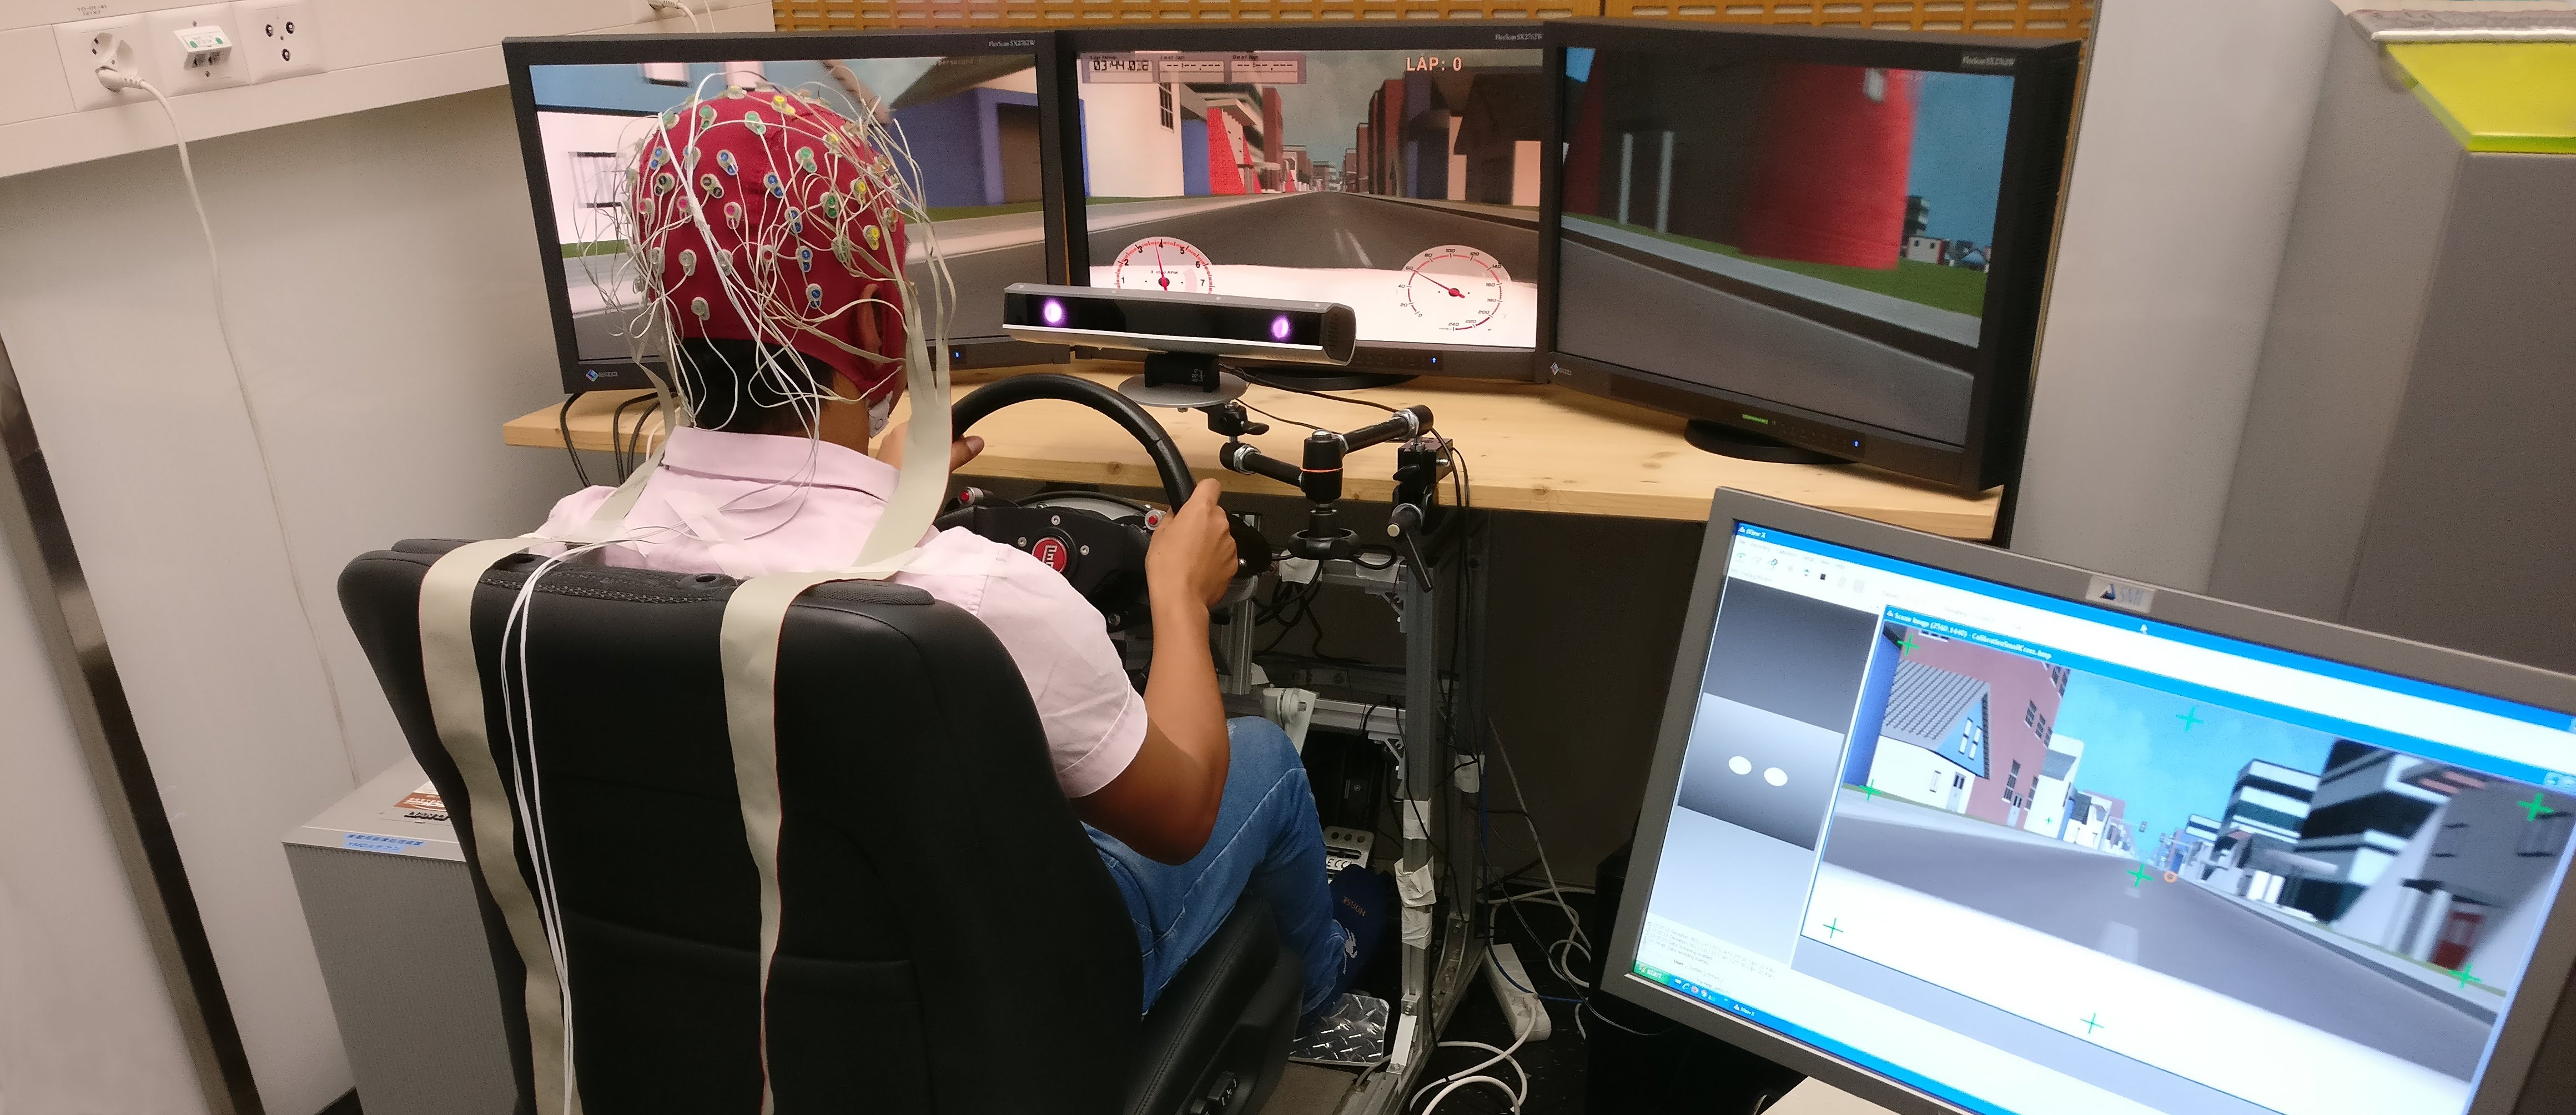
\includegraphics[trim={0cm 0cm 0cm 0cm},clip,width=0.6\columnwidth]{../images/Driving-photo.jpg}
    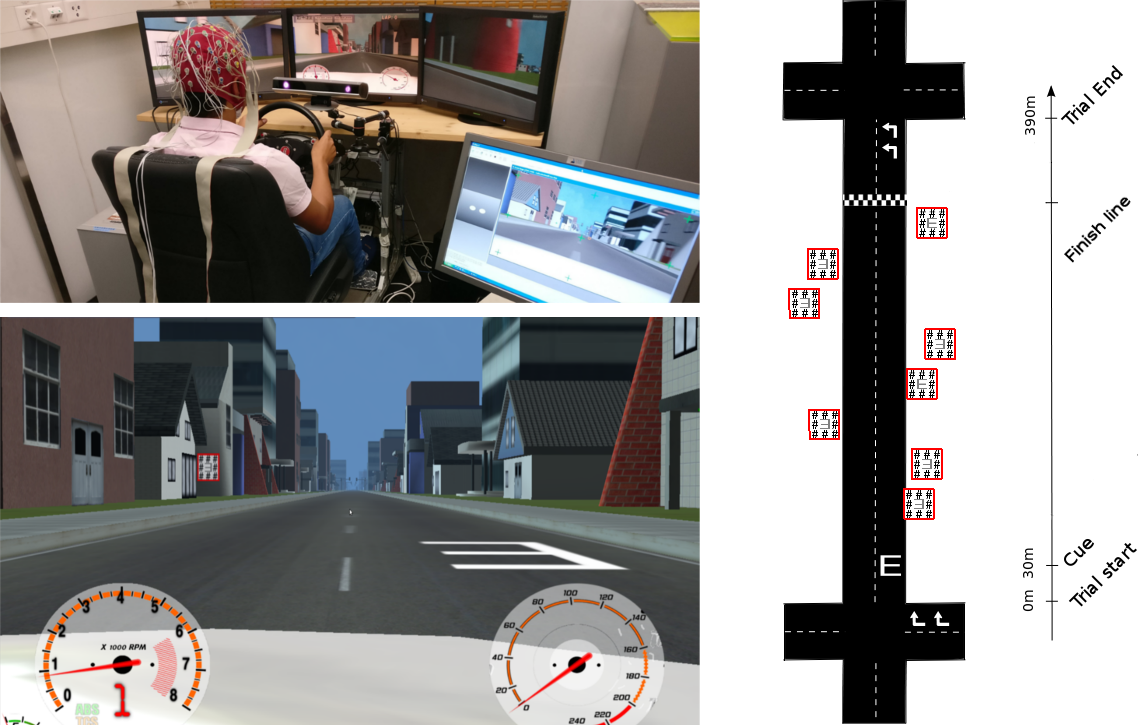
\includegraphics[trim={0cm 0cm 0cm 0cm},clip,width=0.8\columnwidth]{../images/setup_protocol2.png}
    \caption{Experimental setup (top left), screenshot from the beginning of the road (bottom left)
    and schematic drawing of one road (right).}
\label{fig:setup}
\end{figure}

%\begin{figure}[!t]
    %\includegraphics[trim={0cm 0cm 0cm 0cm},clip,width=0.6\columnwidth]{../images/Target}
    %\caption{Protocol}
%\label{fig:protocol}
%\end{figure}

\section{Methods}
\subsection{Objectives}
We split the data processing and analysis into 3 category:
offline, simulated online and online.
The offline data processing is done on the data collected from offline phase
and its purpose is to obtain
a clean dataset for the analysis and the classifier training.
The online data processing is done during the online phase,
thus its outcome demonstrates the application performance.
Since only one decoding approach could be tested in online
phase, we compared several decoding approaches in a simulated online manner.

\label{sec:methods}
\subsection{Fixation extraction and analysis}
There exist numerous methods to extract eye movement events
from the eye gaze direction. Some of them proved to provide
a better quality according to the human experts
however are more challenging to implement in real time.
We used one of the methods for offline analysis and another one
for real-time online processing and simulated online analysis.
Simulated online analysis is implemented identical to online phase.


\subsubsection*{Offline fixation extraction.}
The detection of fixation is done with the Identification by 2-Means Clustering (I2MC) method.
We relied on the implementation provided by the authors of the method
using the default parameters.
The main idea behind is to find the transition between two consecutive fixations
by applying 2-mean clustering in a sliding window manner.
During fixation the eyes do not move so if we can clearly detect
2 clusters it means that they correspond to two fixations.
This method is more precise and robust to noisy outliers which
allows to obtain a training dataset of higher quality.

\subsubsection*{Online and simulated online fixation extraction.}
We could not use the provided implementation of I2MC in real time
to extract fixations so we used the Identification by Dispersion-Threshold (IDT)
supplied with our eye tracking system. Fixation in IDT is extracted
when the signals lies within the dispersion thresholds for at least a minimum fixation duration.
It requires two parameters: we used 100 ms for the minimum fixation duration
and 200 pixels for the maximum dispersion.

\subsubsection*{Fixation analysis.}
The cognitive response is stronger when the stimulus is perceived and recognized
for the first time. We assume that subjects categorized the symbol at the first
attendance so we use only the first fixations on the boards for our analysis.

The visual input during the task is dynamic. Due to driving through
the virtual environment the objects including the boards are also moving on the screen.
So we assume that most of the board attendances are done with
smooth pursuit rather than fixations. 
To the best of our knowledge there is no available algorithm for efficient
extraction of smooth pursuit for eye movement data sampled at 120 Hz.
The only consequence of 
extracting fixation from smooth pursuit is that a single smooth pursuit
may be oversegmented into multiple fixations.
For the sake of our analysis we do not need to differentiate between
fixations and smooth pursuit movement. The onset of first fixation on a board
will coincide with the onset of smooth pursuit.

For the behavioral analysis we estimate the total attendance time of boards
for the first uninterrupted visit or dwell time. The dwells were created
by merging all the fixations on the same board with saccade durations
between them below 50 ms.

Each fixation and dwell were assigned to a target board, a non-target board or non-board.
Due to a reading visual span of several degrees, the board movement and 
noisy eye tracking data we applied the following approach to assign the boards
to fixations. For each eye gaze sample we estimate the probability of
fixating eyes on the center of the board according to a normal distribution.
After averaging log-probabilities across the dwell time we apply a hard
threshold to assign the fixation to a board or a non-board class.


\subsection{EEG processing}
\subsubsection*{EEG processing of offline data.}
All the EEG and EOG were filtered with Butterworth band-pass filter
of order 4 within the band [1, 10] Hz
using noncausal filtering and downsampled from 2 kHz to 256 Hz.
Due to low conductivity of the skull and the skin,
EEG signal is spatially smoothed so a high contrast between nearby channels
is a result of noise and movement artifacts. We remove this noise
by keeping only low spatial frequency components after decomposition EEG with SPHARA.
Horizontal and vertical components of eye movement were estimated which allowed
to remove the eye movement artifacts from EEG using multivariate regression.
The coefficients of multiple regression were estimated from the 
one-minute session of eye movements before the corresponding run.
Then the signal is spatially
filtered with common-average-reference (CAR). 

\subsubsection*{EEG processing in simulated online.}
The EEG processing was identical to the offline analysis
except for the eye movement artifacts removal. The multiple regression
model was obtained from offline data.

\subsubsection*{EEG processing in online.}
The online phase required the real time processing. SMI system provides
a real time eye fixation detection. The fixations were buffered
by a parallel process within the driving simulator, matched with the boards,
and a trigger was sent to the BioSemi system 3 s after the onset of each the fixation
on a board. We choose 3 s delay because we apply non-causal filter on EEG data.
EEG processing  was identical to the offline procedure
except for 2 steps:
\begin{itemize}
    \item the spectral filtering was done on a 5 s buffer of data,
        approximately around [-2, 3] s around the fixation onset;
    \item the eye movement artifacts were removed based on the multiple
        regression coefficients trained with offline phase eye movement data.
\end{itemize}

\subsection{Decoding approaches}
The epochs are extracted
from time window of [200, 1000] ms after the fixation onset.
We investigate and compare different sets
of features, EFRP waveform and covariance-based features.

\subsubsection*{Offline decoding.}
For the offline analysis we chose the following combination of features and classifiers:
\begin{itemize}
    \item \textbf{Linear}. Penalized logistic regression (PLR) trained on waveform features after reducing
        the dimensionality with PCA. Only the components which explain 90\% of variance
        are kept. 
    \item \textbf{Dwell}. PLR trained on dwell time on the boards.
    \item \textbf{Linear with Dwell}. PLR trained on the combination of waveform features with dwell time. We concatenate
        the two feature sets before applying PCA to keep 95\% of variance. Since the dynamic
        range of dwell time in ms is greater than the one of EEG in uV, most of the information
        remains is projecte
    \item \textbf{Random Forest}. Random forest trained on waveform features. We use 100 decision trees and
        with maximum depth of 5.
    \item \textbf{Riemann}. PLR trained on Riemannian features from simple epochs.
        To build Riemannian features we
        estimate spatial covariance matrix with shrinkage and project it
        to the tangent space according to the classical Riemannian geometry on SPD matrices.
        We subselected 8 channels based on mean Fisher score across the epoch.
    \item \textbf{Riemann+}. PLR trained on Riemannian features from augmented epochs.
        Before computing the covariance matrix we augment the epoch with the averaged ERP
        for each class (target and non-target). Otherwise, it is identical to the previous
        approach.
\end{itemize}

Since PLR is a linear regularized classifier we standardize all the features to z-score when
using PLR.

\subsubsection*{Simulated online decoding.}
The EEG processing was identical to the offline analysis
except for the eye movement artifacts removal. The multiple regression
model was obtained from offline data.

\subsubsection*{Online decoding.}
On the data obtained in the offline phase we trained Random Forest classifier
and applied it in real time. The probability for the target class was sent
back to the driving simulator. After crossing the finish line
the probabilities were averaged per each symbol (1 out of 4).
The symbol which had the highest probability of being a target was
shown to the subject on the screen.


\subsection{Performance evaluation}

\subsubsection*{Offline performance evaluation.}
We employ nested cross validation to adjust various hyperparameters in the inner loop:
regularization term for PLR and the tree depth in Random Forest.
The purpose of the outer loop is to obtain an unbiased performance estimation
so it is critical to avoid training and testing on correlated data.
We achieve it by performing leave-one-run-out for the outer loop,
although we had only 3 offline runs.
The inner loop is implemented with 4-fold cross validation while keeping
the temporal order of the trials before the split.
Since the classes of target and non-target eye fixations are unbalanced,
we utilized AUC to measure the classification performance.

\subsubsection*{Simulated online performance evaluation.}
After training the classifiers on all the offline data we applied them 
to all the online data and obtained a single AUC value.

\subsubsection*{Online performance evaluation.}
During online phase we predicted the target symbol from the EFRP classification.
We assess the overall performance with accuracy and confusion matrices
for 4 symbols.

\section{Results}
\label{sec:results}
\subsection{Behavioral analysis}

\subsubsection*{Board attendance}
Subject attended most of the boards in the offline phase and approximately
half of them in the online phase. One of the subjects
had a poor quality of eye tracker calibration which led
to poor fixation extraction. This subject is excluded from the behavioral analysis.
The average attendance rate
is shown in the Table \ref{tab:boardAtt}. 
Repeated measures ANOVA shows significant difference between
all 4 groups: targets in offline, targets  in online,
non-targets in offline and non-targets in online, with $p-value < 0.0001$.
Post-hoc analysis shows that it is driven by the difference between
offline and online phases with p-value $< 0.0001$ (paired t-test).
The difference between targets and non-targets is not significant with p-value $= 0.048$
so we can assume that subjects could not differentiate the symbols
with peripheral vision.

\begin{table}
    \centering
    \caption{Board attendance rate for targets and non-targets in offline and online phases.
    The numbers represent the average and standard deviation across subjects.}
    \begin{tabular}{c | c | c}
        \hline 
        & Offline & Online \\
        \hline 
        Targets & 0.92 $\pm$ 0.07 & 0.47 $\pm$ 0.06 \\
        Non-Targets & 0.92 $\pm$ 0.07 & 0.44 $\pm$ 0.09 \\
        \hline 
    \end{tabular}
    \label{tab:boardAtt}
\end{table}
%TargOff    0.868838
%DistOff    0.865138
%TargOn     0.454746
%DistOn     0.428700

\subsubsection*{Counting}
The total number of targets in offline phase is 173.
We analyzed the button presses which should be equal to the number of targets
on each road.
The average number of incorrect counts (both missed and extra counts) was 5,
the worst performance was at 15 errors (Figure \ref{fig:classAll}).


\subsubsection*{Dwell time}
We analyzed the distribution of dwell times on targets vs non-targets
in offline and online phases (Figure \ref{fig:dwell}). 
Most of the dwells are limited to the time between the boards pop up equal to 900 ms.
The dwell times are identical for non-targets in both phases and significantly
shorter than for targets (p-value $< 0.0001$).
The median dwell time for targets is significantly longer in online phase (p-value $< 0.0001$).

\begin{figure}[!t]
    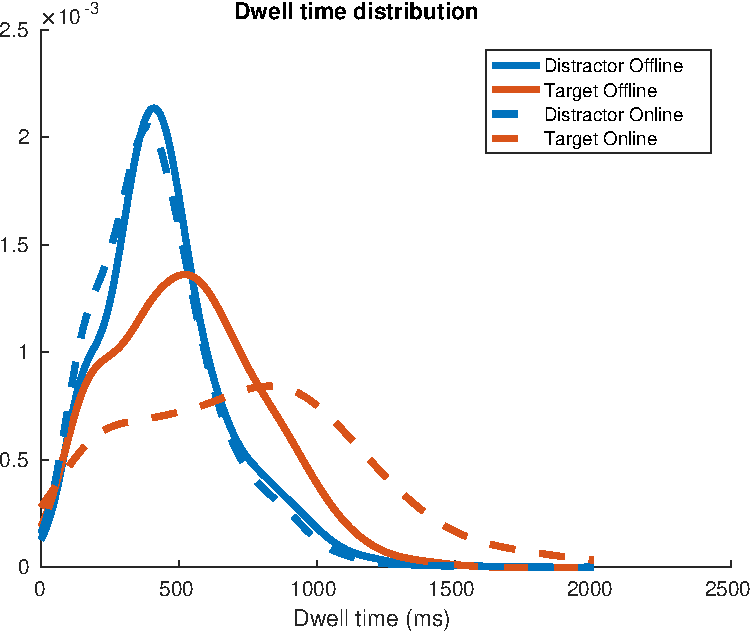
\includegraphics[trim={0cm 0cm 0cm 0cm},clip,width=0.6\columnwidth]{../images/DwelltimeDist_online_allmean.pdf}
    \caption{Dwell time distribution for targets vs distractors in offline and online phases.}
\label{fig:dwell}
\end{figure}

\subsection{EFRP waveform}
\begin{figure}[!t]
    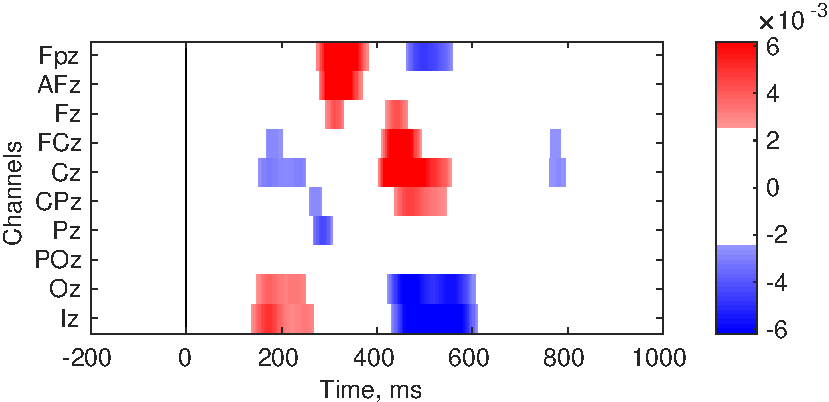
\includegraphics[trim={0cm 0.01cm 0cm 0cm},clip,width=0.45\columnwidth]{../images/SignR_offline.pdf}
    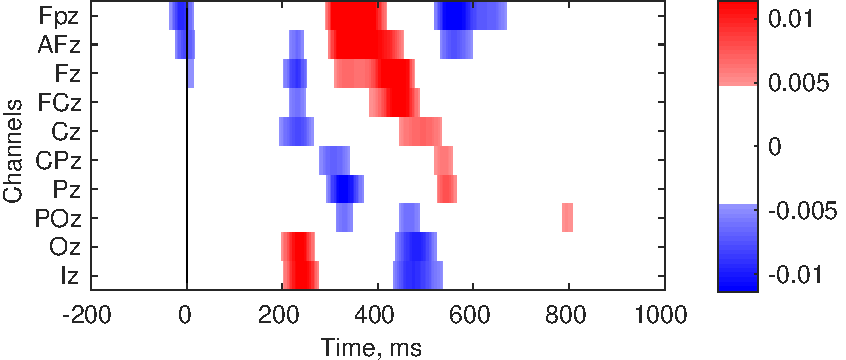
\includegraphics[trim={0cm 0cm 0cm 0.01cm},clip,width=0.45\columnwidth]{../images/SignR_online.pdf}
    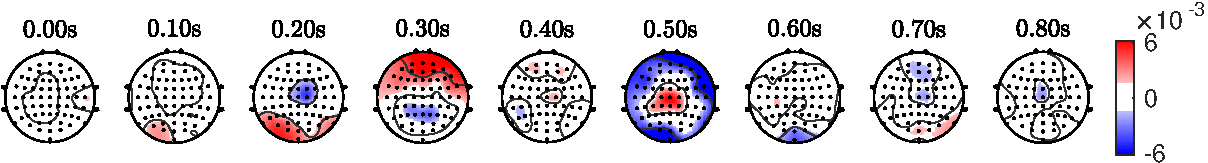
\includegraphics[trim={0cm 0cm 0cm 0cm},clip,width=0.9\columnwidth]{../images/offline/TopoPlot_TLock-start_signRSquare_Saggregate_objrec_subjects_popuponline_s1.pdf}
    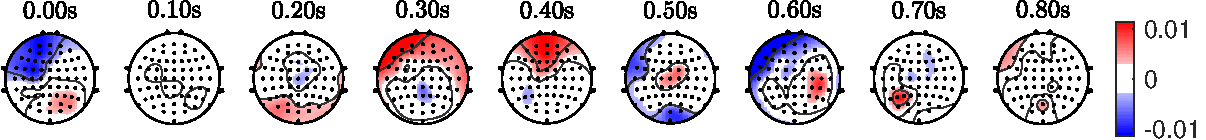
\includegraphics[trim={0cm 0cm 0cm 0cm},clip,width=0.9\columnwidth]{../images/online/TopoPlot_TLock-start_signRSquare_Saggregate_objrec_subjects_popuponline_s1.pdf}
    \caption{The discriminant power for the 4 best subjects with the offline AUC above 60.
    Signed $R^2$ is demonstrated for midline channels across around the eye fixation onset
    (top left: offline, top right: online) and on topographic maps (top map: offline, bottom map: online).}
\label{fig:signR}
\end{figure}

\begin{figure}[!t]
    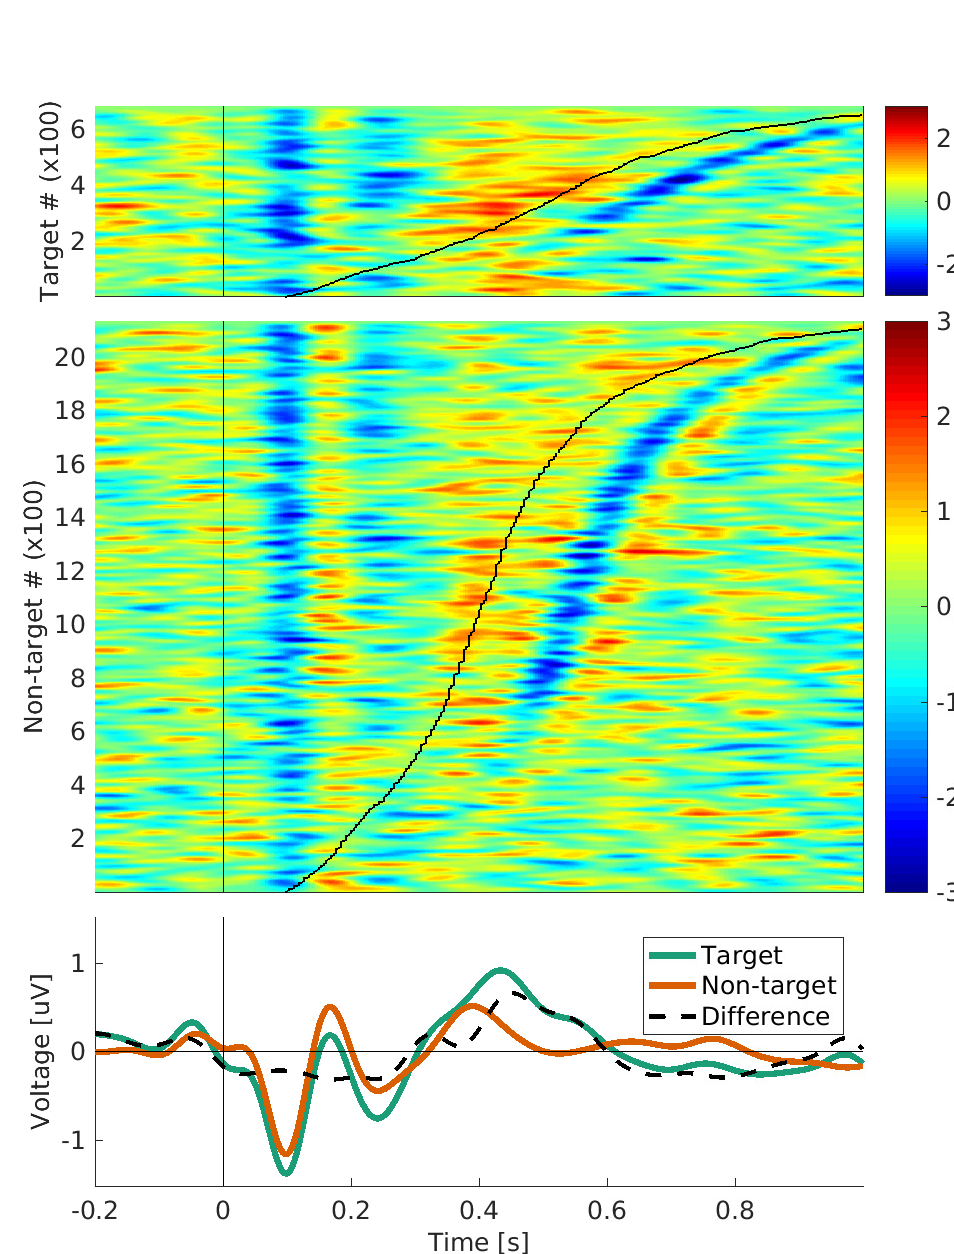
\includegraphics[trim={0cm 0cm 1.5cm 0cm},clip,width=0.45\columnwidth]{../images/offline/Epochs_GA_chCz_Saggregate_objrec_subjects_popuponline_s1.pdf}
    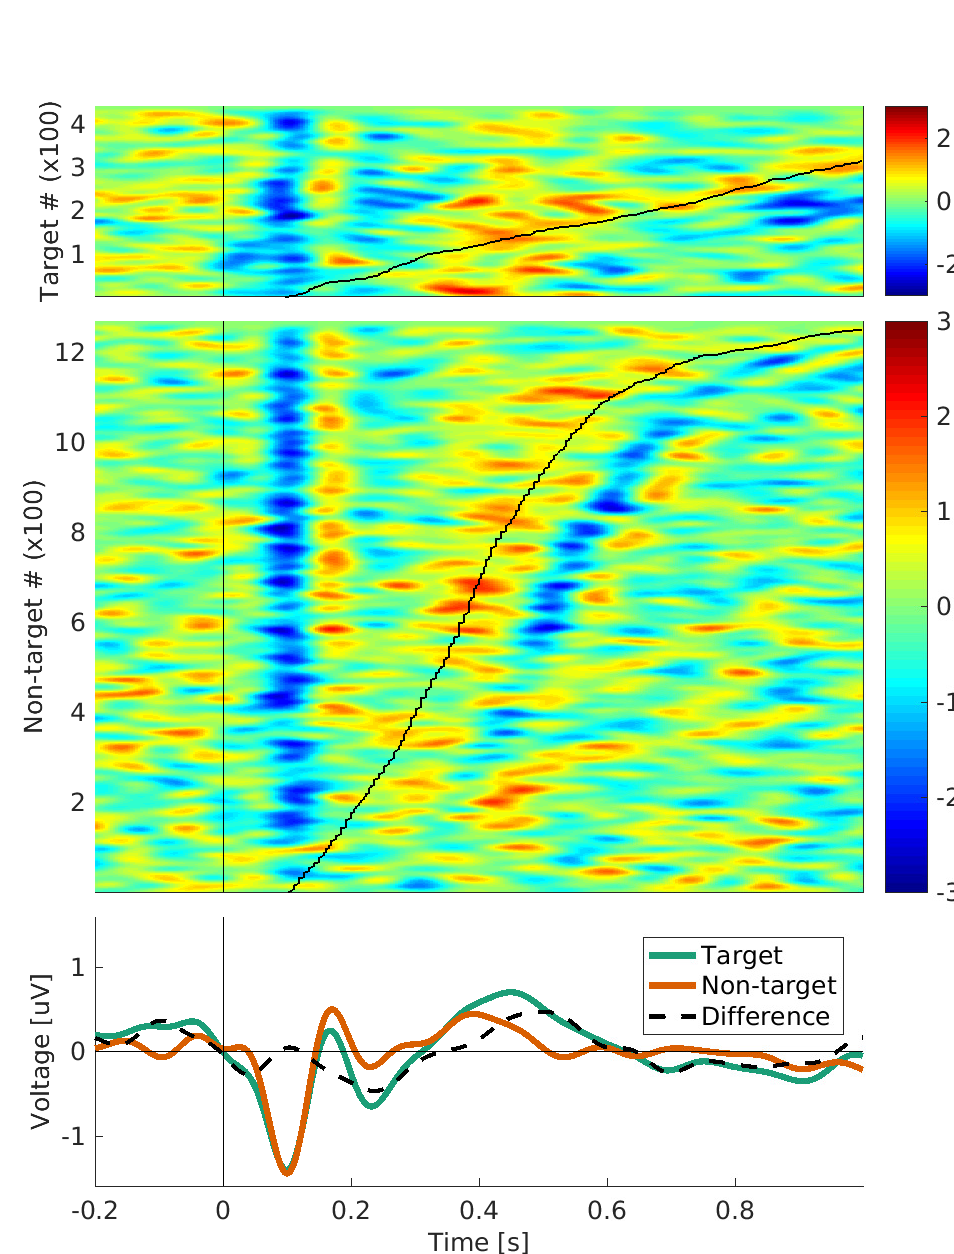
\includegraphics[trim={0cm 0cm 1.5cm 0cm},clip,width=0.45\columnwidth]{../images/online/Epochs_GA_chCz_Saggregate_objrec_subjects_popuponline_s1.pdf}
    \caption{The signal of Cz channel for all epochs for the 4 best subjects. Left: offline, Right: online.
        The black curve shows the offset of the fixation.
    }
\label{fig:epochsCz}
\end{figure}

We present the analysis of the EFRP waveform for the 4 subjects who demonstrated
the highest classification performance in the offline phase with the Linear classifier.
The univariate discriminant power is shown on the Figure \ref{fig:signR}.
The results are similar for the offline and online phases with online data having twice
as higher discriminant power with up to 0.01 of signed $R^2$.
The greatest values are mainly confined within the region between 100 and 700 ms.
The higher discriminant power is spread across the whole scalp which can be the consequence
of using CAR in the processing. Nonetheless, the P300-like component can be seen at 500 ms
after the fixation onset. The representative channel for this component is Cz.

We visualized Cz signal for each eye fixation while ordering them
by the dwell time (Figure \ref{fig:epochsCz}).
The amplitude of the presented EFRP is limited to the range [-1.5, 1.5] uV.
The complex of components right after the fixation onset ranging from 100 to 300 ms
reflects the evoked potentials from the fixation itself. It contains
negative and positive deflections. We can observe the same complex of components
after the dwell offset. The shift of gaze happens right where we expect 
the P300-like component so it can be masked by this evoked activity.
The positive deflection occurs at the end of the dwell for both
targets and non-targets, however it has a greater amplitude for targets
as seen on the averaged EFRP.


\subsection{Comparison of decoding approaches}

\begin{figure}[!t]
    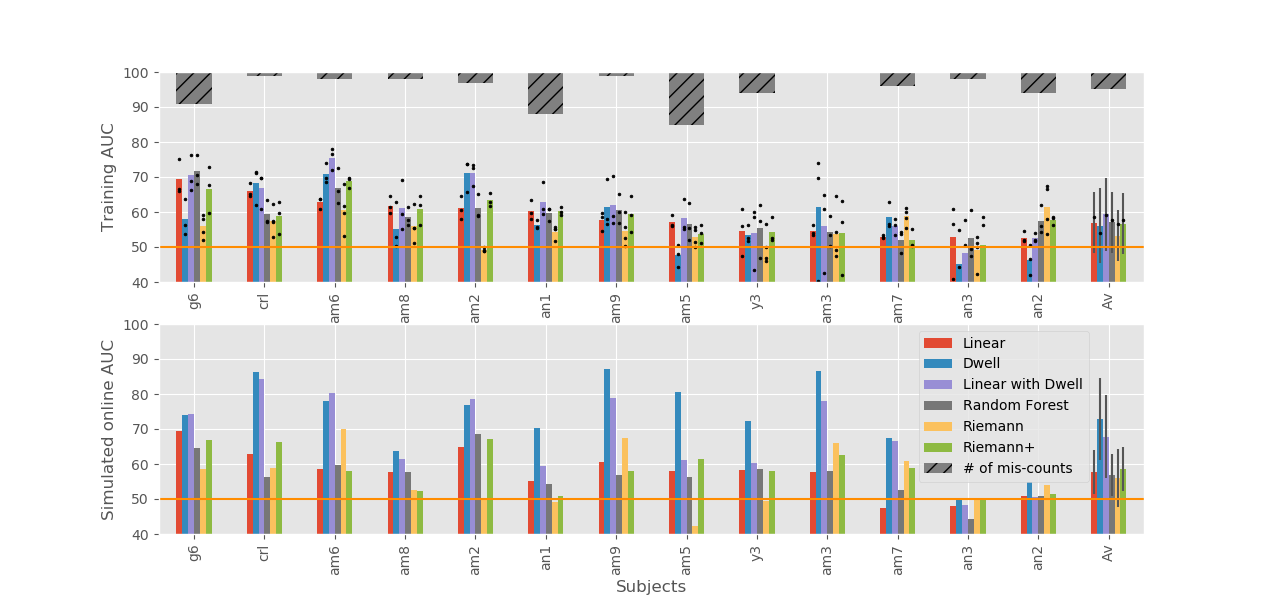
\includegraphics[trim={2cm 0cm 2cm 0cm},clip,width=1.1\columnwidth]{../images/ClassificationAll.png}
    \caption{Performance of EFRP classification with various approaches in offline analysis (top)
    and simulated online analysis (bottom). Each dot shows single fold performance
    in a leave-one-run-out cross validation for the corresponding classification approach.}
\label{fig:classAll}
\end{figure}

\subsubsection*{Offline}
All the classification approaches lead to the performance between 53 and 60 AUC points on average
(Figure \ref{fig:classAll})
which is statistically significant against random level of 50 
(p-values $< 0.001$ with Student's t-test after Bonferroni correction).
Eight out of thirteen subjects achieve performance above 60 for at least one of the approaches based
on neural correlates.
Performance of different approaches has a different ranking per subject, however
the differences between
the approaches are not statistically significant (p-value $= 0.16$ with repeated measures ANOVA).
It is worth noticing that the combination of both dwell time and EEG waveform is not always
better than just one of these feature sets.

\subsubsection*{Simulated online}
First of all, we note that the performance of neural-based approaches 
on online data is consistent with the training performance on offline data.
The average AUC values lie between 56 and 59 for each approach
which is statistically significant against 50
(p-values $< 0.001$ with Student's t-test after Bonferroni correction).

For approaches relying on the dwell time, however, the performance drastically improved
for multiple subjects. The average AUC for \textit{dwell} classifier increased
from 56 to 73 and for the \textit{Linear with Dwell} classifier from 59 to 67.
This improvement is a direct consequence of the changes in target dwell time
together with the constant non-target dwell time shown in \ref{fig:dwell}.


\subsection{Online performance}

\begin{figure}[!t]
    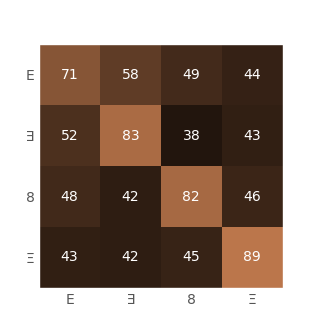
\includegraphics[trim={0cm 0cm 0cm 0cm},clip,width=0.5\columnwidth]{../images/OnlineConfusion.png}
    \caption{The aggregated confusion matrix of online decoding for each type of symbol being
    a target.}
\label{fig:onlineconf}
\end{figure}


\begin{table}
    \centering
    \caption{Online performance}
    %\tiny
    %\footnotesize
    \scriptsize
    \renewcommand{\arraystretch}{1.5}
    \begin{tabular}{l r r r r r r r r r r r r r}
        \hline
        Subjects & S1 & S2 & S3 & S4 & S5 & S6 & S7 & S8 & S9 & S10 & S11 & S12 \\
        \hline

        Accuracy & 0.44 & 0.38 & 0.45 & 0.29 & 0.44 & 0.35 & 0.39 & 0.25 & 0.31 & 0.38 & 0.38 & 0.4 \\ 
        %0.44, 0.38, 0.45, 0.29, 0.44, 0.35, 0.39, 0.25, 0.31, 0.38, 0.38, 0.4
        \shortstack{Accuracy \\ test} & \textbf{0.003} & 0.29 & \textbf{0.002} & 5.27 & \textbf{0.003} & 0.62 & 0.08 & 12.0 & 2.40 & 0.29 & 0.29 &
        0.16 \\
        \shortstack{Independence \\ test}  & \textbf{ 0.004} & 2.58 & 0.06 & 8.91 & 0.24 & 0.84 & 0.39 & 4.13 & 5.26 & 1.14 & 1.53
        & 2.07 \\
        \hline
        %Binom:  [0.003, 0.2903, 0.0016, 5.2731, 0.003, 0.6192, 0.0771, 12.0, 2.4047, 0.2903, 0.2903, 0.1592]
        %Chi * 12  [0.0044, 2.5806, 0.0608, 8.9126, 0.243, 0.8449, 0.3913, 4.1269, 5.2593, 1.1424, 1.5352, 2.0768]
    \end{tabular}
    \label{tab:onlineperf}
\end{table}

We assessed the task performance of each subject as the accuracy of
target decoding (Table \ref{tab:onlineperf}). The averaged accuracy 
equals 0.37 and it is significantly different from random level of 0.25 for
a classification of 4 between balanced classes (p-value $< 0.0001$ with Student's t-test).
Additionally, we applied statistical test to assess the accuracy per subject.
After Bonferroni correction only 3 subjects performed statistically better than random performance.

To verify the independence of the 4 classes in online phase
we computed the aggregated confusion matrices across all symbol (Figure \ref{fig:onlineconf}).
We applied an independence test for confusion matrices per subject.
After Bonferroni correction only one subject shows significant imbalance in the
confusion matrix. It is linked to a high accuracy of the symbol $\Xi$ and low accuracy 
for the symbol E.


\section{Discussion}
\label{sec:discussion}
Decoding of cognitive process from EFRP has a potential to augment
real life interaction with machines for healthy users.
However, there are still challenges to solve to achieve
a satisfactory performance.

In this study we investigated the scenario of simulated driving.
We limit the driving task to following the simple route at a comfortable and natural speed
without other participants of the traffic or other moving objects.
However, due to the movement of the car, the drivers
were subjected to a dynamic visual input. Although subjects followed
the objects moving on the screen,
we could analyze their eye behavior by approximating smooth pursuit
with consecutive fixations combination.

In the online phase subjects looked longer on targets compared to the offline phase.
Although the subjects dwell time was not decoded directly, they were aware
that they could potentially influence the decoding quality. This might
lead to deliberate or unconscious changes in their behavior.
Some subjects could achieve a high decoding performance based
only on dwell time in offline phase. But with the changes in the behavior
during online phase most of the subjects drastically improve in their decoding performance.

We observed a statistically significant difference in the board attendance
between offline and online phases. On one hand, we expected the subjects to 
be more engaged in the task due to interactive feedback part.
Observed longer dwells on targets make it more challenging to attend
all the boards.
On the other hand, behavioral reports were not required which released
the pressure to complete the task properly.

Comparing targets vs non-targets we found no difference in the attendance rate
which confirms that subjects could recognize the symbol only by directly looking at it.
The behavioral reports show that subjects properly counted the number
of targets on the road with a limited number of errors.
So most of the board attendances led to a proper recognition in the offline phase.
Moreover, the balanced confusion matrices in the online phase
confirm that subjects perceived all the symbols equally with the regards
to the task. The presence of new types of stimuli did not alter
the cognitive process.

The discriminant analysis of EFRP shows similar results for both
offline and online phases. Most of the relevant
features lie within [200, 700] ms window which coincides with the dwell
durations. The spatial localization of relevant features is consistent with the typical
spatial distribution of P300 component in oddball paradigm.
The EFRP waveforms are known to contain a strong P1 component at the occipital
area that reflects the beginning of the visual processing of a stable visual input
after the saccade. In the analysis of Cz channel it corresponds to the negative
deflection at 100 ms. It is clearly present in most of the fixations on boards.
Moreover, we could also see it for the following fixations.
It leads to the overlap between P300-like component and 
the evoked fixation-related components. This overlap contaminates the
data and complicates the decoding of cognitive process.
Removing the evoked activity from the EEG can be done
by modeling it from various characteristics of the previous fixations and saccades \cite{nikolaev_combining_2016}.
However, there is a risk to remove the cognitive signal even with EFRP collected
from more controlled conditions with static visual input.

We limited the removal of artifacts to high frequency spatial noise with SPHARA 
and direct eye movement potential propagation by regressing it out 
from the EOG signal.

We compared multiple classification approaches based on EFRP on offline data and 
simulated their application to online data.
All approaches including waveform-based linear and non-linear and covariance-based 
methods result in similar performance on average across subjects
which is significantly above the chance level.
However there is no single best approach for all subjects.

One can argue that the high performance of EFRP-based classifiers is
due to the strong and well-aligned evoked potentials after the fixations,
which reflects the difference between the target and non-targets dwell times.
In this case we would see an improvement in performance for online data
similar to the classification approaches based on dwell time.
The combination of two sources of information (EEG and dwell time), nonetheless,
does not lead to significant improvement and in the simulated online
decoding it results in intermediate performance.

The actual online performance measured by the target symbol identification
is significantly above the chance level only for 3 subjects.
Nonetheless, on average across subjects the accuracy of 0.37 is 
significantly higher than 0.25.



\section*{References}

\bibliographystyle{unsrt}
\bibliography{ObjRec_DS.bib}

\end{document}

